% !TeX program = xelatex
% Meeting Follow-up Slides #4 -- Gary Wang
% Simplified: key figures + brief notes

\documentclass[aspectratio=169]{beamer}

\usepackage{graphicx}
\graphicspath{
    {../}
    {./Figures/}
    {../Figures/}
    {../../feature_selection/fs_results/png/}
    {../../feature_selection/traditional_fs_results/plots/}
    {../../experiments_llmlasso/results/}
}
\makeatletter
\def\input@path{{../}{./}}
\makeatother

\mode<presentation>{
    \usetheme{NordlingLab169}
}

\usepackage[english]{babel}
\let\latinencoding\relax
\usepackage{xltxtra}
\setsansfont{Candara}

\usepackage[yyyymmdd]{datetime}
\renewcommand{\dateseparator}{--}

\usepackage{booktabs}
\usepackage{xcolor}
\usepackage{tikz}
\usetikzlibrary{arrows.meta, positioning}

\title[Meeting Follow-up \#4]{Progress Update \#4:\\Feature Selection Pipeline}
\author[Gary Wang]{Gary Wang}
\institute[NCKU]{Nordling Lab @
    Dept.\ of Mechanical Engineering\\
    National Cheng Kung University}
\date{\today}

\begin{document}

\setbeamertemplate{background}[NLTitle]
\setbeamertemplate{footline}[NLTitle]
\begin{frame}
    \titlepage
\end{frame}

\setbeamertemplate{background}[NLCC]
\setbeamertemplate{footline}[NLCC]

%%%%%%%%%%%%%%%%%%%%%%%%%%%%%%%%%%%%%%%%%%%%%%%%%%%%%
\begin{frame}
    \frametitle{Pipeline Overview}
    \centering
    \scalebox{0.85}{%
    \begin{tikzpicture}[
        node distance=0.6cm,
        box/.style={rectangle, rounded corners, draw, thick,
                    minimum width=9cm, minimum height=0.9cm, align=center},
        arr/.style={-Stealth, thick},
    ]
        \node[box, fill=blue!10]   (s1) {\textbf{Stage 1:} 17 FS methods $\to$ each outputs a 0/1 mask};
        \node[box, fill=orange!10, below=of s1] (s2) {\textbf{Stage 2:} 3 predictors (KNN, SVR, RF) $\times$ LOOCV $\to$ MAE, Kappa, \dots};
        \node[box, fill=green!10,  below=of s2] (s3) {\textbf{Stage 3:} Rank features by inclusion frequency (good FS only)};
        \node[box, fill=red!10,    below=of s3] (s4) {\textbf{Stage 4:} Feed top-$K$ features to LLM (32B) $\to$ find best $K$};
        \draw[arr] (s1) -- (s2);
        \draw[arr] (s2) -- (s3);
        \draw[arr] (s3) -- (s4);
    \end{tikzpicture}}
\end{frame}

%%%%%%%%%%%%%%%%%%%%%%%%%%%%%%%%%%%%%%%%%%%%%%%%%%%%%
\begin{frame}
    \frametitle{Amplitude Normalisation Fixed (min-max)}
    \centering
    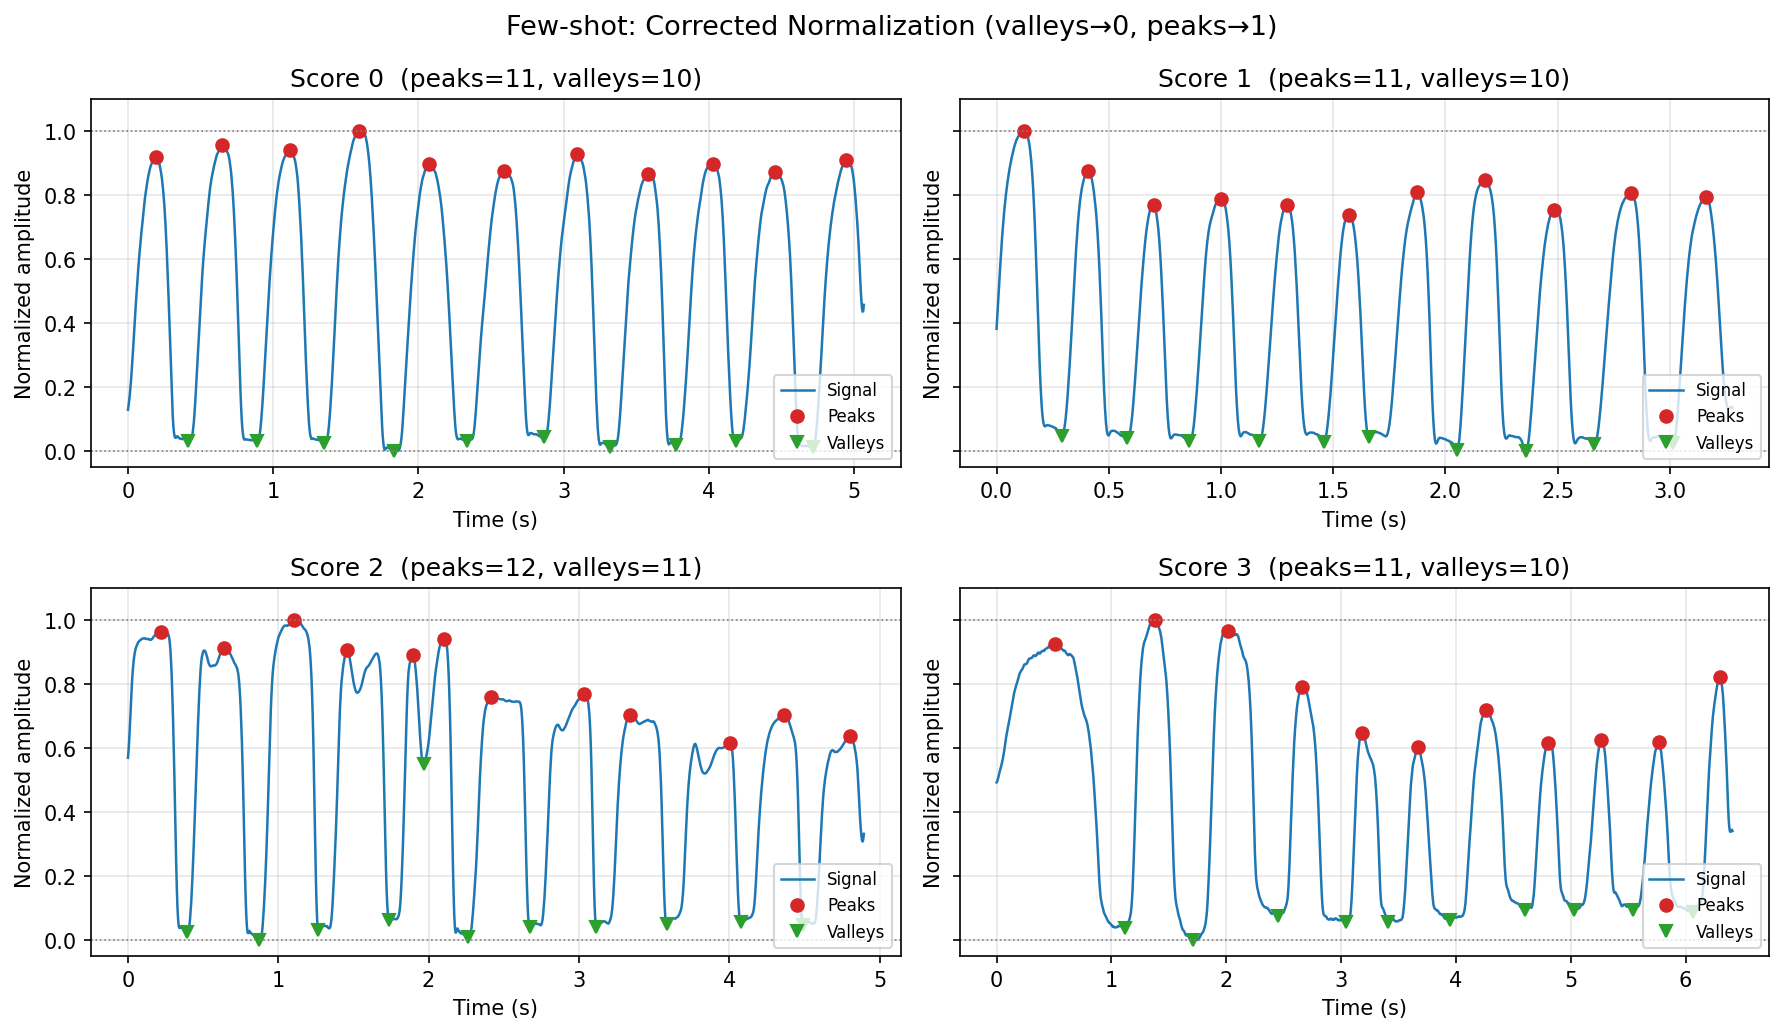
\includegraphics[width=0.48\textwidth,height=0.75\textheight,keepaspectratio]{fewshot_amplitude_corrected_signal.png}\hfill
    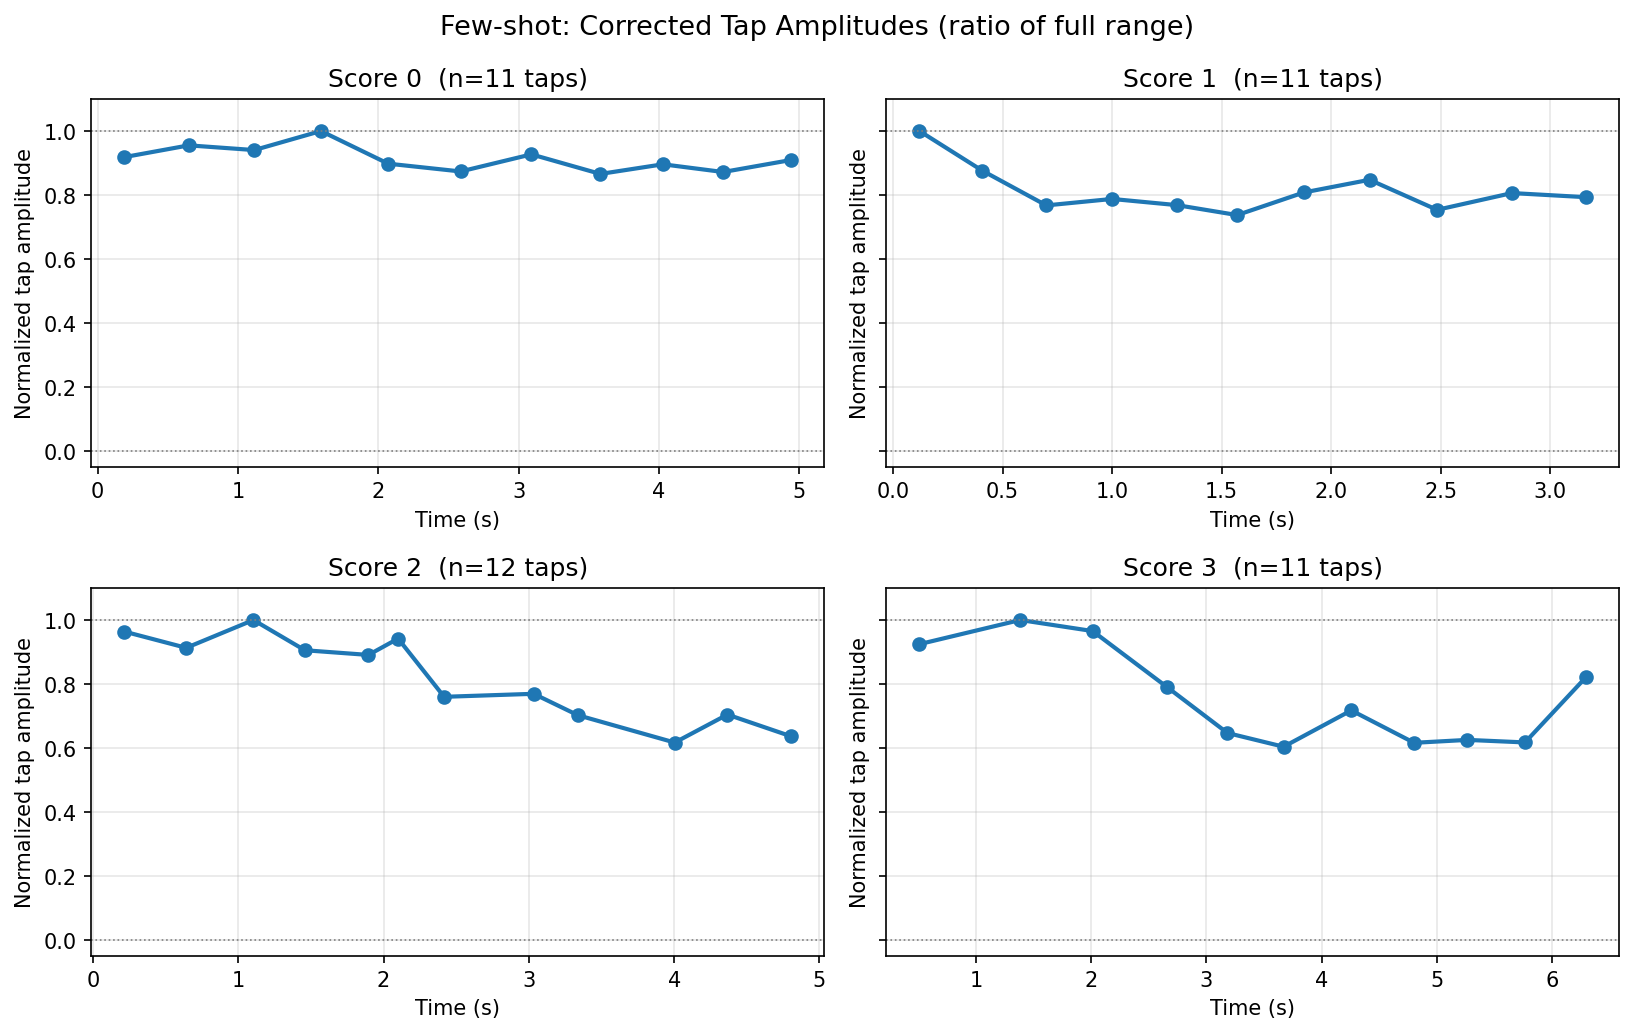
\includegraphics[width=0.48\textwidth,height=0.75\textheight,keepaspectratio]{fewshot_amplitude_corrected_taps.png}
    \\[0.2em]
    \scriptsize Lowest valley now $= 0$, highest peak $= 1$ (advisor's fix from Meeting \#4).
\end{frame}

%%%%%%%%%%%%%%%%%%%%%%%%%%%%%%%%%%%%%%%%%%%%%%%%%%%%%
\begin{frame}
    \frametitle{Stage 1: Which Method Picks Which Features}
    \centering
    
\includegraphics[width=\textwidth,height=0.82\textheight,keepaspectratio]{feature_overlap_heatmap.png}
    \\[0.1em]
    \scriptsize Each row = one FS method. Yellow cell = feature selected.
\end{frame}

%%%%%%%%%%%%%%%%%%%%%%%%%%%%%%%%%%%%%%%%%%%%%%%%%%%%%
{
\setbeamertemplate{background}{}
\setbeamertemplate{footline}{}
\setbeamertemplate{headline}{}
\begin{frame}[plain]
    \frametitle{Stage 2: \#Features vs.\ Kappa Trade-off}
    \centering
    
\includegraphics[width=\textwidth,height=0.88\textheight,keepaspectratio]{figD_nfeats_vs_kappa.png}
    \\[0.1em]
    \scriptsize Keep FS methods with \textbf{Kappa $\geq 0.5$} and \textbf{\#features $<15$}
    (bottom-right region)
\end{frame}
}

%%%%%%%%%%%%%%%%%%%%%%%%%%%%%%%%%%%%%%%%%%%%%%%%%%%%%
\begin{frame}
    \frametitle{Stage 3: Feature Ranking (Good FS Only)}
    \centering
    
\includegraphics[width=0.9\textwidth]{figE_feature_frequency.png}
    \\[0.3em]
    \footnotesize Count only among FS methods with Kappa $\geq 0.5$ and \#feat $<15$.
\end{frame}

%%%%%%%%%%%%%%%%%%%%%%%%%%%%%%%%%%%%%%%%%%%%%%%%%%%%%
\begin{frame}
    \frametitle{Key Responses to Meeting \#4}
    \small
    \begin{itemize}
        \item \textbf{Amplitude normalisation}: ratio-to-max $\to$ min-max
              (min = 0, max = 1).
        \item \textbf{No artificial grouping}: every FS method sees the same
              scalar feature matrix.
        \item \textbf{Evaluation defined}: 3 predictors $\times$ LOOCV $\times$
              4 metrics --- uniform across all FS methods.
        \item \textbf{LLM cost}: 32B LLM reserved for Stage 4 only;
              cheap surrogates handle Stage 2.
    \end{itemize}
\end{frame}

%%%%%%%%%%%%%%%%%%%%%%%%%%%%%%%%%%%%%%%%%%%%%%%%%%%%%
\begin{frame}
    \frametitle{Open Question}
    \centering
    \large
    How should the per-tap amplitude sequence be represented?\\[1em]
    \normalsize
    \begin{tabular}{ll}
        \textbf{(A) Per-position} & \texttt{tap\_amp\_norm\_01..20} --- 20 individual features\\[0.3em]
        \textbf{(B) Summary} & \texttt{amplitude\_median}, \texttt{amp\_cv},
                               \texttt{decrement\_slope}, \dots\\
    \end{tabular}
    \\[1em]
    \footnotesize
    Most FS methods can only accept scalar columns --- favouring (B).
\end{frame}

\begin{frame}
    \frametitle{Thank You}
    \centering
    \vspace{1em}
    \Large Questions \& Feedback\\[1em]
    \normalsize gary.wang@nordlinglab.org
\end{frame}

\end{document}
